\documentclass[9pt]{beamer}
\usetheme{Warsaw}
\usefonttheme[onlymath]{serif}

\usepackage[utf8]{inputenc}
%\usepackage[polish]{babel}
\usepackage[T1]{fontenc}
\usepackage{comment}
\usepackage{setspace}
\usepackage{amsmath}
\usepackage{dcolumn}
\usepackage{siunitx}
\usepackage{tabularx}
\usepackage{graphicx}
\graphicspath{{../images/}}

\sisetup{
    table-number-alignment = center, % Align numbers at the decimal point
    table-format = +1.4e3,           % Specify number format: 1 digit before, 3 after decimal, and 1 exponent
    tight-spacing = true,           % Remove extra spacing around numbers
}

\newcolumntype{M}{>{\centering\arraybackslash\math}p{2cm}}

\newcommand{\n}{\newline}

\linespread{1}

\title{Projekt 1, Zadanie 23}
\author{Wiktor Murawski, 333255, grupa 3, środa 12:15}
\date{}


\begin{document}

\begin{frame}
    %\frametitle{\insertauthor,\space\inserttitle}

    \begin{spacing}{1.75}
    \begin{center}
        \inserttitle\par
        \insertauthor
    \end{center}
    \vspace{2em}
    Obliczanie całek $ \iint\limits_D f(x,y) \, dxdy $ na obszarze
    $  D = \{(x,y) \in \mathbb{R}^2 : |x| + |y| \leq 1\} $
    poprzez podział obszaru $ D $ na $ 4n^2 $ trójkątów przystających oraz
    zastosowanie na każdym z nich kwadratury rzędu drugiego.
    \end{spacing}
\end{frame}


\begin{frame}
\frametitle{Podział obszaru $D$ na $4n^2$ trójkątów przystających}
    \begin{columns}
        \column{0.5\textwidth}
        \centering
        Podział $D$ dla $n = 1$\\
        \vspace{1em}
        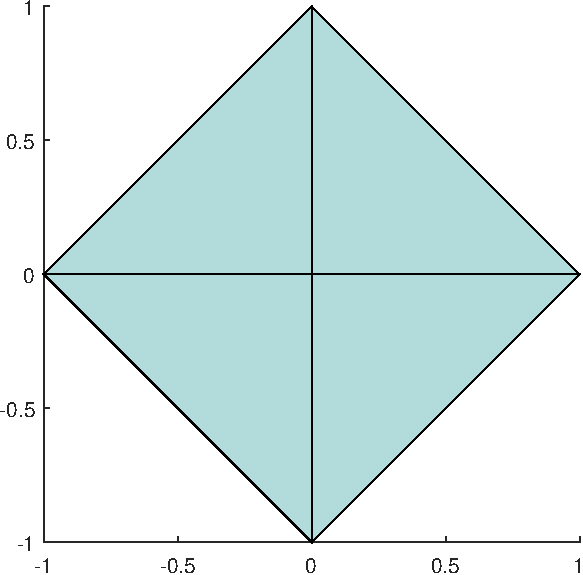
\includegraphics[width=\textwidth]{figure1.pdf}


        \column{0.5\textwidth}
        \centering
        Podział $D$ dla $n = 4$\\
        \vspace{1em}
        \includegraphics[width=\textwidth]{figure4.pdf}

    \end{columns}
\end{frame}


\begin{frame}
    TU MA BYĆ ALGORYTM
\end{frame}


\begin{frame}
    \frametitle{Formuła całkowa na trójkącie}
    Niech $T$ będzie trójkątem o wierzchołkach $(x_1,y_1), (x_2,y_2), (x_3,y_3) \in \mathbb{R}^2$
    Niech $P$ oznacza pole trójkąta $T$ oraz niech 
    $$ A = \begin{pmatrix}
    	1 & 1 & 1 \\
    	x_1 & x_2 & x_3 \\
    	y_1 & y_2 & y_3 \\
    \end{pmatrix} $$
    Wtedy $$P = \frac{1}{2}|\det{A}|$$
    Niech $f : \mathbb{R}^2 \to \mathbb{R}$. Wówczas 
    $$S_S(f) = P f \left(\frac{x_1+x_2+x_3}{3},\frac{y_1+y_2+y_3}{3} \right) $$
    $$S_W(f) = \frac{P}{3} \Big( f(x_1,y_1) + f(x_2,y_2) + f(x_3,y_3) \Big)$$
    są kwadraturami rzędu 2-go.
    
\end{frame}

\begin{frame}
	 \begin{spacing}{1.5}
	Mając podział obszaru $ D $ na $4 n^2 $ trójkątów przystających oraz kwadraturę drugiego rzędu na dowolnym trójkącie, możemy obliczyć całkę $$ I(f) = \iint\limits_D f(x,y)  \, dxdy $$ poprzez zastosowanie na każdym z trójkątów kwadratury rzędu drugiego.\\
	
	Stosując kwadraturę $ S_S(f) $ na każdym z trójkątów, 
	otrzymamy kwadraturę złożoną $ S_S^{[n]}(f) $.\\
	
	Spodziewamy się, że dla dostatecznie dużego $ n $
	$$ S_S^{[n]} \approx I(f) $$	
	a dla wielomianów dwóch zmiennych stopnia $ < 2 $
	$$ S_S^{[n]} = I(f) $$ 

	\end{spacing}
\end{frame}

\begin{frame}
\frametitle{Sprawdzanie poprawności}

    \begin{spacing}{1}
        W celu sprawdzenia poprawności metody przetestujemy ją na wielomianach dwóch zmiennych stopnia pierwszego.\par
        Obliczymy analitycznie 
        $$ I = \iint\limits_D f(x,y) \, dx dy $$ 
        gdzie
        $$ f(x,y) = ax + by + c \qquad a,b,c \in \mathbb{R}$$
        Niech 
        $$ D_1 = \{(x,y) \in D : x \leq 0\} $$ 
        $$ D_2 = \{(x,y) \in D : x > 0\} $$ 
        Oznaczmy 
        $$ I_1 = \iint\limits_{D_1} f(x,y) \, dx dy $$ 
        $$ I_2 = \iint\limits_{D_2} f(x,y) \, dx dy $$ 
        Wtedy $ D = D_1 \cup D_2 $ oraz $ I = I_1 + I_2 $.
        %$$ I_1 = \int\limits_{-1}^{0}\int\limits_{-x-1}^{x+1} ax+by+c \, dy dx $$
        %$$ I_2 = \int\limits_{0}^{1}\int\limits_{x-1}^{-x+1} ax+by+c \, dy dx $$
    \end{spacing}

\end{frame}

\begin{frame}
\frametitle{Wyznaczenie analityczne całki z funkcji stopnia 1}
    \begin{columns}
        \begin{column}{0.5\textwidth}
            % Lewa kolumna
            \begin{align*}
                I_1 &= \int\limits_{-1}^{0}\int\limits_{-x-1}^{x+1} ax+by+c \,dydx \\
                I_1 &= \int\limits_{-1}^{0}\left[axy + \frac{by^2}{2} + cy\right]_{-x-1}^{x+1} \,dx \\
                I_1 &= \int\limits_{-1}^{0} 2ax^2 + 2ax + 2cx + 2c \,dx \\
                I_1 &= 2\left[ \frac{ax^3}{3} + \frac{ax^2}{2} + \frac{cx^2}{2} + cx \right]_{-1}^{0} \\
                I_1 &= -\frac{a}{3} + c \\
            \end{align*}
        \end{column}
        \begin{column}{0.5\textwidth}
            % Prawa kolumna
            \begin{align*}
                I_2 &= \int\limits_{0}^{1}\int\limits_{x-1}^{-x+1} ax+by+c \,dydx \\
                I_2 &= \int\limits_{0}^{1}\left[axy + \frac{by^2}{2} + cy\right]_{x-1}^{-x+1} \,dx \\
                I_2 &= \int\limits_{0}^{1} - 2ax^2 + 2ax - 2cx + 2c \,dx \\
                I_2 &= 2\left[ -\frac{ax^3}{3} + \frac{ax^2}{2} - \frac{cx^2}{2} + cx \right]_{0}^{1} \\
                I_2 &= \frac{a}{3} + c \\
            \end{align*}
        \end{column}
    \end{columns}

    \begin{center}
        Ostatecznie otrzymujemy $ I = I_1 + I_2 = 2c $
    \end{center}
\end{frame}

\begin{frame}
	\frametitle{Testy poprawności}
	\begin{table}[]
		\makebox[\linewidth]{
			\begin{tabular}{|l|S|l|S|S|}
				\hline & & & & \\[-1em]
				Funkcja $f$  & {$ I(f) $} &{$n$}& {$S_S^{[n]}(f)$} & {$|S_S^{[n]}(f) - I(f)|$}\\
				\hline & & & &\\[-1em]
				%---------------------------------------------------------------------------				
$f(x,y) = $                  & 2.0000e+00 & 1   & 2.0000e+00 & 0.0000e+00 \\%0.0000e+00
$ 1 $                      &            & 5   & 2.0000e+00 & 1.3323e-15 \\%6.6613e-16
				             &            & 10  & 2.0000e+00 & 2.0650e-14 \\%1.0325e-14
				             &            & 50  & 2.0000e+00 & 1.8763e-13 \\%9.3814e-14
				             &            & 100 & 2.0000e+00 & 2.0082e-12 \\%1.0041e-12
			                 &            & 500 & 2.0000e+00 & 1.5836e-11 \\%7.9181e-12
				%---------------------------------------------------------------------------
				\hline & & & &\\[-1em]
				%---------------------------------------------------------------------------
$f(x,y) = $                  & 2.0000e+00 & 1   & 2.0000e+00 & 0.0000e+00 \\%0.0000e+00
$ x + y + 1 $                &            & 5   & 2.0000e+00 & 8.8818e-16 \\%4.4409e-16
				             &            & 10  & 2.0000e+00 & 2.4425e-15 \\%1.2212e-15
				             &            & 50  & 2.0000e+00 & 4.6629e-15 \\%2.3315e-15
				             &            & 100 & 2.0000e+00 & 4.8850e-15 \\%2.4425e-15
				             &            & 500 & 2.0000e+00 & 7.5939e-14 \\%3.7970e-14
				%---------------------------------------------------------------------------
				\hline & & & &\\[-1em]
$f(x,y) = $                  & 1.0000e+00 & 1   & 1.0000e+00 & 0.0000e+00 \\%0.0000e+00
$ 8x+2y+\frac{1}{2}$         &            & 5   & 1.0000e+00 & 5.5511e-16 \\%5.5511e-16
			                 &            & 10  & 1.0000e+00 & 2.2204e-16 \\%2.2204e-16
		                     &            & 50  & 1.0000e+00 & 1.1102e-15 \\%1.1102e-15
			                 &            & 100 & 1.0000e+00 & 1.7764e-15 \\%1.7764e-15
			                 &            & 500 & 1.0000e+00 & 8.2157e-15 \\%8.2157e-15
				\hline
			\end{tabular}
		}
	\end{table}
\end{frame}

\begin{frame}
	\frametitle{Testy poprawności}
	\begin{table}[]
		\makebox[\linewidth]{
			\begin{tabular}{|l|S|l|S|S|}
				\hline & & & & \\[-1em]
				Funkcja $f$  & {$ I(f) $} &{$n$}& {$S_S^{[n]}(f)$} & {$|S_S^{[n]}(f) - I(f)|$}\\
				\hline & & & &\\[-1em]
				%---------------------------------------------------------------------------				
$ f(x,y) = $                 &  2.8284e+00 & 1   &  2.8284e+00 & 0.0000e+00 \\%0.0000e+00  
$ x-y+\sqrt2$              &             & 5   &  2.8284e+00 & 1.3323e-15 \\%4.7103e-16  
                             &             & 10  &  2.8284e+00 & 1.7764e-15 \\%6.2804e-16  
                             &             & 50  &  2.8284e+00 & 5.3291e-15 \\%1.8841e-15  
                             &             & 100 &  2.8284e+00 & 3.0198e-14 \\%1.0677e-14  
                             &             & 500 &  2.8284e+00 & 1.5543e-14 \\%5.4953e-15  

				%---------------------------------------------------------------------------
				\hline & & & &\\[-1em]
				%---------------------------------------------------------------------------
$ f(x,y) = $                 & -6.2832e+00 & 1   & -6.2832e+00 & 0.0000e+00 \\%-0.0000e+00  
$ -x + 2y - \pi $          &             & 5   & -6.2832e+00 & 8.8818e-16 \\%-1.4136e-16  
                             &             & 10  & -6.2832e+00 & 0.0000e+00 \\%-0.0000e+00  
                             &             & 50  & -6.2832e+00 & 3.5527e-15 \\%-5.6543e-16  
                             &             & 100 & -6.2832e+00 & 4.4409e-15 \\%-7.0679e-16  
                             &             & 500 & -6.2832e+00 & 3.5527e-14 \\%-5.6543e-15  


				%---------------------------------------------------------------------------
				\hline & & & &\\[-1em]
$ f(x,y) = $                 &  0.0000e+00 & 1   &  0.0000e+00 & 0.0000e+00 \\%NaN  
$ \pi x - ey $               &             & 5   &  1.3878e-17 & 1.3878e-17 \\%Inf  
                             &             & 10  & -6.9389e-18 & 6.9389e-18 \\%Inf  
                             &             & 50  &  9.7578e-19 & 9.7578e-19 \\%Inf  
                             &             & 100 &  1.3281e-18 & 1.3281e-18 \\%Inf  
                             &             & 500 &  7.9028e-19 & 7.9028e-19 \\%Inf  

				\hline
			\end{tabular}
		}
	\end{table}
\end{frame}

\begin{frame}
    TESTY NUMERYCZNE
\end{frame}


\begin{frame}
    TU MA BYĆ WYKRES
\end{frame}


\end{document}
